\section{Begriffsdefinition des (Wortes) Informationsmanagements - BH}
\textit{Autor: Boris Heiliger}

Im Folgenden soll das Informationsmanagement im Allgemeinen erklärt werden, auf die Besonderheiten von Hochschulen wird in den späteren Kapiteln genauer eingegangen.

Das Informationsmanagement ist ein Bestandteil der Unternehmensführung und hat planende, kontrollierende und steuernde Aufgaben sowohl im strategischen als auch im operativen Bereich zu erfüllen. Zudem soll es die Entscheidungsprozesse in den Unternehmen oder Organisationen, in denen Informationsmanagement eingesetzt wird, mit den nötigen Informationen zu versorgen. Informationen sollten im Rahmen des Informationsmanagements also als Ressource angesehen werden, die im Unternehmen gesammelt, verarbeitet und genutzt werden kann.\footnote{\cite[65-68]{voss_informationsmanagement_2001}}

Grob lässt sich Informationsmanagement in drei Aufgabenbereiche unterteilen. Zum einen hat es die Klärung und Planung des \textbf{Informationsbedarfs} zur Aufgabe, in der abgewägt werden muss, welche Informationen (Qualität), wann (Dringlichkeit) und in welchem Umfang (Quantität) benötigt werden.

Ist der Informationsbedarf geklärt, muss die \textbf{Informationsbeschaffung} geplant 
und organisiert werden. Hier stellt sich die Frage, wo (Ort, Quelle, Medium), wie (Werkzeuge), wann (im günstigsten Moment) und durch wen (Qualifikation, Fähigkeiten) die Informationen beschafft werden können.

Sind die Informationen beschafft, folgt die \textbf{Informationssicherung, Nutzbarmachung und Nutzenmehrung}. Hier müssen die Informationen aufbereitet (Aus- und Bewerten), verarbeitet (Integrieren und Kombinieren), präsentiert (vor einer entsprechenden Zielgruppe) und dokumentiert (Archivieren) werden.\footnote{\url{http://www.dr-luepke.de/Seiten/InfoMangmt1.htm}, abgerufen am 23.05.2015}

\subsection{Begriffsdefinition Information}

\textbf{Unterschiedung zwischen Informationen, Daten und Wissen}
Laut Probst umfasst Wissen Konzepte, Erfahrung und Einsichten und bezeichnet damit die Gesamtheit personengebundener Kenntnisse und Fähigkeiten, welche zur Problemlösung eingesetzt werden. Dabei stützt sich Wissen auf Daten (gegebene Inhalte) und Informationen.\footnote{\cite{probst_wissen_2006}}

Laut Wittmann ist Information zweckorientiertes Wissen. Zweckorientiert bedeutet in diesem Fall, dass nur solches Wissen als Information bezeichnet wird, das für das Treffen von Entscheidungen oder Handlungstätigkeiten dient.\footnote{\cite{wittmann_unternehmung_1959}}

\textbf{Information als Produktionsfaktor}
Wie schon weiter oben erwähnt, ist es wichtig, Informationen als wertschöpfenden Faktor für den unternehmerischen Erfolg einschätzen zu können. Für die Produktion von Gütern oder auch für die Bereitstellung von Dienstleistungen sind Informationen notwendig, die Auskunft darüber geben, welche Elemente wo und in welcher Qualität beschafft werden können und wie diese z.B. verarbeitet werden müssen.\footnote{\cite{bode_informationsbegriff_1997}}

Informationen im Sinne des Informationsmanagements sind demnach also immaterielle Güter, die beliebig zu vervielfältigen sind. Es sind jedoch keine freien Güter, da sie einen monetären Wert haben, der von der kontextspezifischen und zeitlichen Verwendung abhängt.\footnote{\cite{krcmar_informationsmanagement_2015}}

Informationen verbrauchen sich bei Nutzung nicht bzw. nutzen sich nicht ab, sind leicht erweiterbar und können schnell und einfach transportiert werden.\footnote{\cite{teubner_information_2005}}

\textbf{Lebenszyklus von Informationen}
Informationen unterliegen des weiteren einem Informationslebenszyklus. Dieser beschreibt, wie ein Informationsbedürfnis entsteht und anschließend die Planung für ein Informationssystem erfolgt. Ist das Informationssystem erstellt, wird es in den laufenden Betrieb integriert und für den Anwender nutzbar gemacht. Entsteht ein neues Informationsbedürfnis, kann später das veraltete Informationssystem durch ein Neues ersetzt werden.\footnote{(\cite{dippold_datenmanagement_2005})}

\begin{figure}[h!]
	\centering
	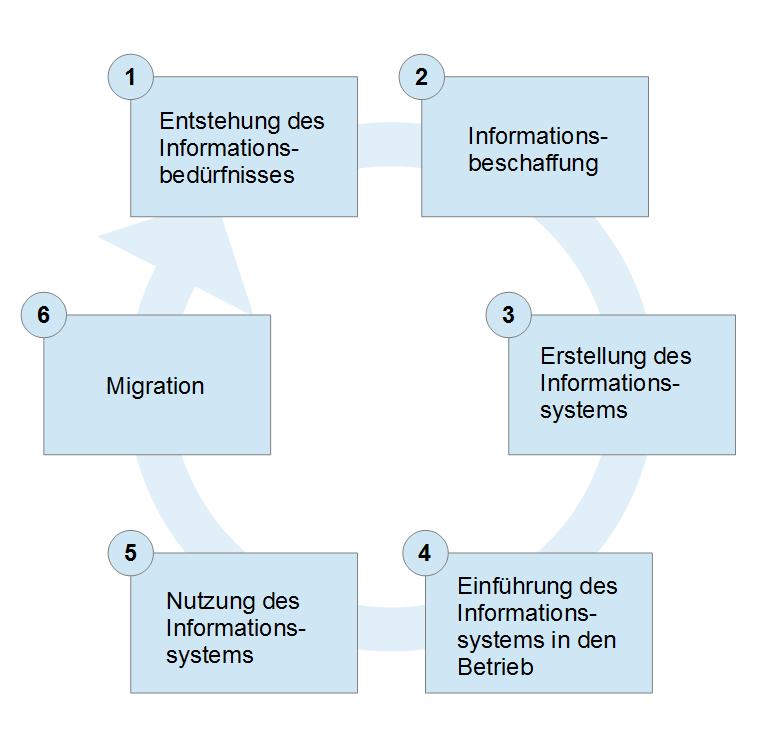
\includegraphics[width=10cm]{kapitel/gruppe1_1/bilder/informations-lebenszyklus}
	\caption{Informations-Lebenszyklus}
	\label{fig_informations_lebenszyklus}
\end{figure}

Ich bin ein Satz, der sich auf Abbildung \ref{fig_informations_lebenszyklus} bezieht und die Quelle dazu angibt.\footnote{Was ist meine Quelle?}

\subsection{Informationsmanagementmodell in der Literatur}
In der deutschsprachigen Literatur lassen sich viele verschiedene Arbeiten und Definitionen zum Thema Informationsmanagement finden, die sich zum Teil deutlich voneinander unterscheiden. Im Folgenden wollen wir kurz auf die Informationsmanagementmodelle- und Sichtweisen von Heinrichs, Wollnik und Krcmar eingehen.

\subsection{Informationsmanagement nach Heinrich}

Lange Zeit stellte das 1987 erschienene Werk von Lutz Heinrich das deutschsprachige Standardwerk im Bereich des Informationsmanagement dar.\footnote{\cite{heinrich_informationsmanagement_2005}} Entsprechend wurde es auch als Lehrbuch an Hochschulen eingesetzt.\footnote{\cite{heinrich_inm_2002}}

Laut Heinrich wird unter Informationsmanagement das “Leitungshandeln (Management) im Unternehmen im Bezug auf Information und Kommunikation” verstanden.\footnote{\cite{heinrich_informationsmanagement_2005}}

Es umfasst alle Führungsaufgaben, die sich mit Information und Kommunikation befassen. Diese Informations- und Kommunikationsaufgaben werden als Informationsfunktion bezeichnet, die den Schwerpunkt des Informationsmanagements darstellt. 

Das Ziel des Informationsmanagements laut Heinrich ist es, eine Informationsinfrastruktur aufzubauen, die die Verteilung, Produktion und Nutzung vom Informationen zur Aufgabe hat. Die Informationsinfrastruktur dient dazu, das Leistungspotenzial der Informationsfunktion umzusetzen und somit einen optimaler Beitrag zum Unternehmenserfolg zu leisten.\footnote{\cite{heinrich_inm_2002}}

Für die Umsetzung der Ziele werden die Aufgaben des Informationsmanagements in drei Ebenen strukturiert.
Die \textbf{strategische} Ebene plant, überwacht uns steuert die Informationsinfrastruktur.
Die \textbf{administrative} Ebene plant, überwacht und steuert die Komponenten der Informationsinfrastruktur (z.B. Anwendungssysteme, Mitarbeiter, Bestand an Daten).
Die \textbf{operative} Ebene umfasst Aufgaben und Nutzung der Informationsinfrastruktur. Mögliche Aktionsfelder für die operative Aufgabenebene stellen den laufenden Betrieb, die Nutzerunterstützung und die Störungsbeseitigung dar.

Auf jeder Aufgabenebene werden Methoden, Techniken und Werkzeuge eingesetzt, die die Durchführung der strategischen, administrativen und operativen Aufgaben durchführt und unterstützt.
Die Gesamtheit dieser Methoden und Techniken wird von Heinrich als \emph{Information Engineering} bezeichnet.

\subsection{Informationsmanagement nach Wollnik}
Michael Wollnik\footnote{\cite{wollnik_referenzmodell_1988}} gliedert das Informationsmanagement in drei Ebenen.

Die \textbf{Ebene des Informationseinsatzes} und dessen Management befasst sich mit der Integration von Informationen in Produkte und Dienstleistungen. Des weiteren befasst es sich mit der Erschließung neuer Märkte durch den Einsatz von Informationstechnologie.

Die \textbf{Ebene der Informations- und Kommunikationssysteme} stellt die mittlere Managementebene dar. Laut Wollnik bestehen Informationssysteme aus folgenden Elementen/Komponenten: Aufgaben, Informationen, Personen, Geräte, Organisation und Programme. Diese bestimmen die Struktur eines Informationssystems. Die Aufgaben dieser Ebene sind die Festlegung, Erhaltung und Modifikation dieser Strukturen während des Lebenszyklus des Informationssystems.

Ein weiteres Handlungsobjekt dieser Ebene sind die Prozesse zur Gestaltung von Informationssystemen, die geplant, organisiert und kontrolliert werden müssen. Diese Ebene stellt das Verbindungsglied zwischen den betrieblichen Aufgaben (Ebene Eins) und der technischen Infrastruktur (Ebene Drei) dar.

Die \textbf{Ebene der Informations- und Kommunikationsinfrastruktur} ist die unterste der drei Ebenen und befasst sich mit der Informationstechnologie. 
Dazu zählt laut Wollnik die Hard- und Software sowie die inhaltlichen Strukturen (zentrale Informationsbestände, Zugriffsberechtigungen auf Informationen). Kernaufgabe dieser Ebene ist der Betrieb und die Entwicklung der Infrastrukturen.\\

Diese drei Ebenen sind hierarchisch strukturiert und stellen den jeweils übergeordneten Ebenen Dienstleistungen zur Verfügung bzw. stellen Anforderungen an die jeweils untergeordneten Ebenen. 

\begin{figure}[h!]
	\centering
	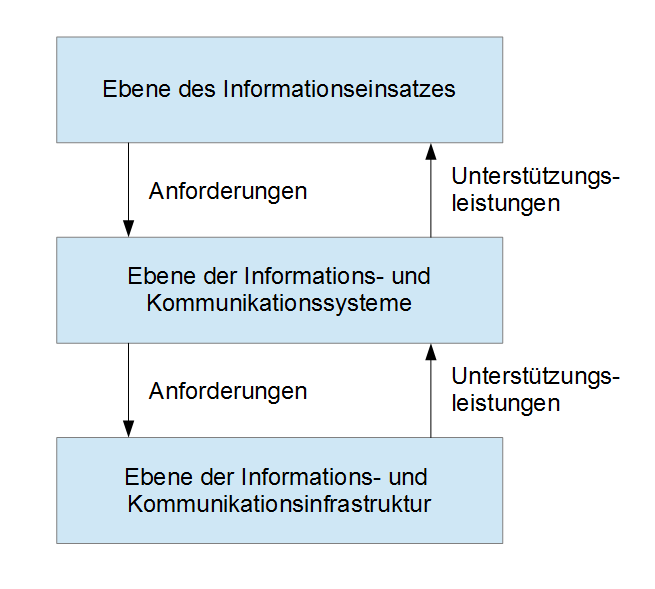
\includegraphics[width=10cm]{kapitel/gruppe1_1/bilder/ebenenmodell_wollnik}
	\caption{Ebenenmodell nach Wollnik}
	\label{fig_ebenenmodell_wollnik}
\end{figure}

Dieses einfache Ebenenmodell stellt auch die Grundlage für viele weitere Informationsmanagementmodelle dar, unter anderem das von Krcmar.

\subsection{Informationsmanagement nach Krcmar}
Krcmars Strukturierung des Informationsmanagement basiert auf dem Ebenenmodell von Wollnik, erweitert es jedoch um allgemeine Führungsaufgaben mit ebenenübergreifenden Funktionen (IT-Governance, Strategie, IT-Prozesse, IT-Personal, IT-Controlling).\footnote{\cite{krcmar_informationsmanagement_2015}}

Er gliedert das Informationsmanagement in die drei Teilbereiche Informationswirtschaft, Informationssysteme und Informations- und Kommunikationstechnik.

Die \textbf{Informationswirtschaft} beschäftigt sich mit dem Angebot, der Nachfrage und Verwendung von Informationen.
Die \textbf{Informationssysteme} haben das Management von Daten, Prozessen und dem Anwendungslebenszyklus zur Aufgabe.
Die \textbf{Informations- und Kommunikationstechnik} weisen die Speicherung, Verarbeitung und Kommunikation von Information als Basisfunktionalitäten auf.

In Kapitel \ref{section_inm_nach_krcmar} wird genauer auf den Aufbau des Informationsmanagementmodells von Krcmar eingegangen.

Da Krcmar mit seinen Publikationen zum Thema Informationsmanagement breiter aufgestellt ist als andere Autoren und er entsprechend oft zitiert wird, soll er auch in dieser Arbeit als Quelle für die nachfolgenden Kapitel sein. 

\subsection{Ziele des Informationsmanagements}
Das Informationsmanagement verfolgt zwei grundlegende Zielsetzungen.
Das erste Ziel ist die Koordination der Informationslogistik bzw. die Gewährleistung der adressatengerichteten Informationsversorgung.
Das zweite Ziel ist die Unterstützung der Unternehmensziele durch eine zielgerichtete und wirtschaftliche Steuerung der Informatik.\footnote{\cite{zarnekow_intergriertes_2004}}

Die Aufgaben des Informationsmanagements leiten sich aus diesen Zielen ab und werden im diesem Kapitel näher beleuchtet.

\subsection{Koordination der Informationslogistik}
In erster Linie ist das Ziel des Informationsmanagements, tatsächlich relevante Information von der Menge an verfügbaren und eventuell unnützen Informationen zu trennen, die für einen Entscheidungsprozess benötigt werden. Hierzu muss jedoch erst einmal ein Informationsbedarf vorliegen, der die Art, Menge und Beschaffenheit der Informationen bestimmt und auf dessen Grundlage eine Entscheidung getroffen werden kann.

Die Definition des Informationsbedarfs hängt einerseits vom Entscheider, andererseits von den Anforderungen der zu treffenden Entscheidung ab.

Der Informationsbedarf lässt sich grundsätzlich in zwei Kategorien einteilen: in den objektiven und den subjektiven Informationsbedarf.\footnote{\cite{picot_grenzenlos_2003}}

Der \textbf{objektive} Informationsbedarf wird in erster Linie durch die Entscheidung festgelegt und baut auf der Aufgabenbeschreibung des Entscheiders und den jeweiligen Marktgegebenheiten auf.
Der \textbf{subjektive} Informationsbedarf wird primär durch den Entscheider festgelegt. Welche Informationen für die Entscheidung relevant sind, werden durch die Einschätzungen und Präferenzen des Entscheiders mitbestimmt.

Aus der Überschneidung des objektiven und subjektiven Informationsbedarfs entsteht die Informationsnachfrage, die wiederum maßgeblich vom Informationsangebot abhängt. Somit legt der Informationsbedarf

\begin{itemize}
	\item die Beschaffenheit (Qualität),
	\item den Zeitpunkt der Lieferung,
	\item den Ort, an dem geliefert wird und
	\item das Medium, über das geliefert wird		 
\end{itemize}
in Bezug auf die Information fest. Im Hinblick auf die Unternehmensziele sollten die Informationen als Ressource angesehen werden.\footnote{\cite{bode_informationsbegriff_1997}} 

\subsection{Informationsmanagement als Unterstützung der Unternehmensziele}
Das Informationsmanagement bildet einen Teil der Unternehmensführung ab, der die Steuerung der Informatik (d.h. Mitarbeiter, Prozesse, organisatorische Teilbereiche und die eingesetzten Informationstechnologien) zur Verantwortung hat.

Die Rahmenbedingungen für die Informationslogistik werden so gestaltet, dass diese Informatik und deren Leistungen auf die Unternehmensziele ausgerichtet ist.\footnote{\cite{voss_informationsmanagement_2001}}

Dazu sollte eine geeignete und zweckorientierte Informationsinfrastruktur (Systemdenken, Rationalisierung, Orientierung am Beschaffungs- und Absatzmarkt) bereitgestellt werden.\footnote{\cite{Vgl. u.a. Vieweger, Bernd; Informationsmanagement; 2013}}
\todo[inline]{Quelle genau bezeichnen, Angaben ungenügend}
